\begin{figure}%
	\centering%
	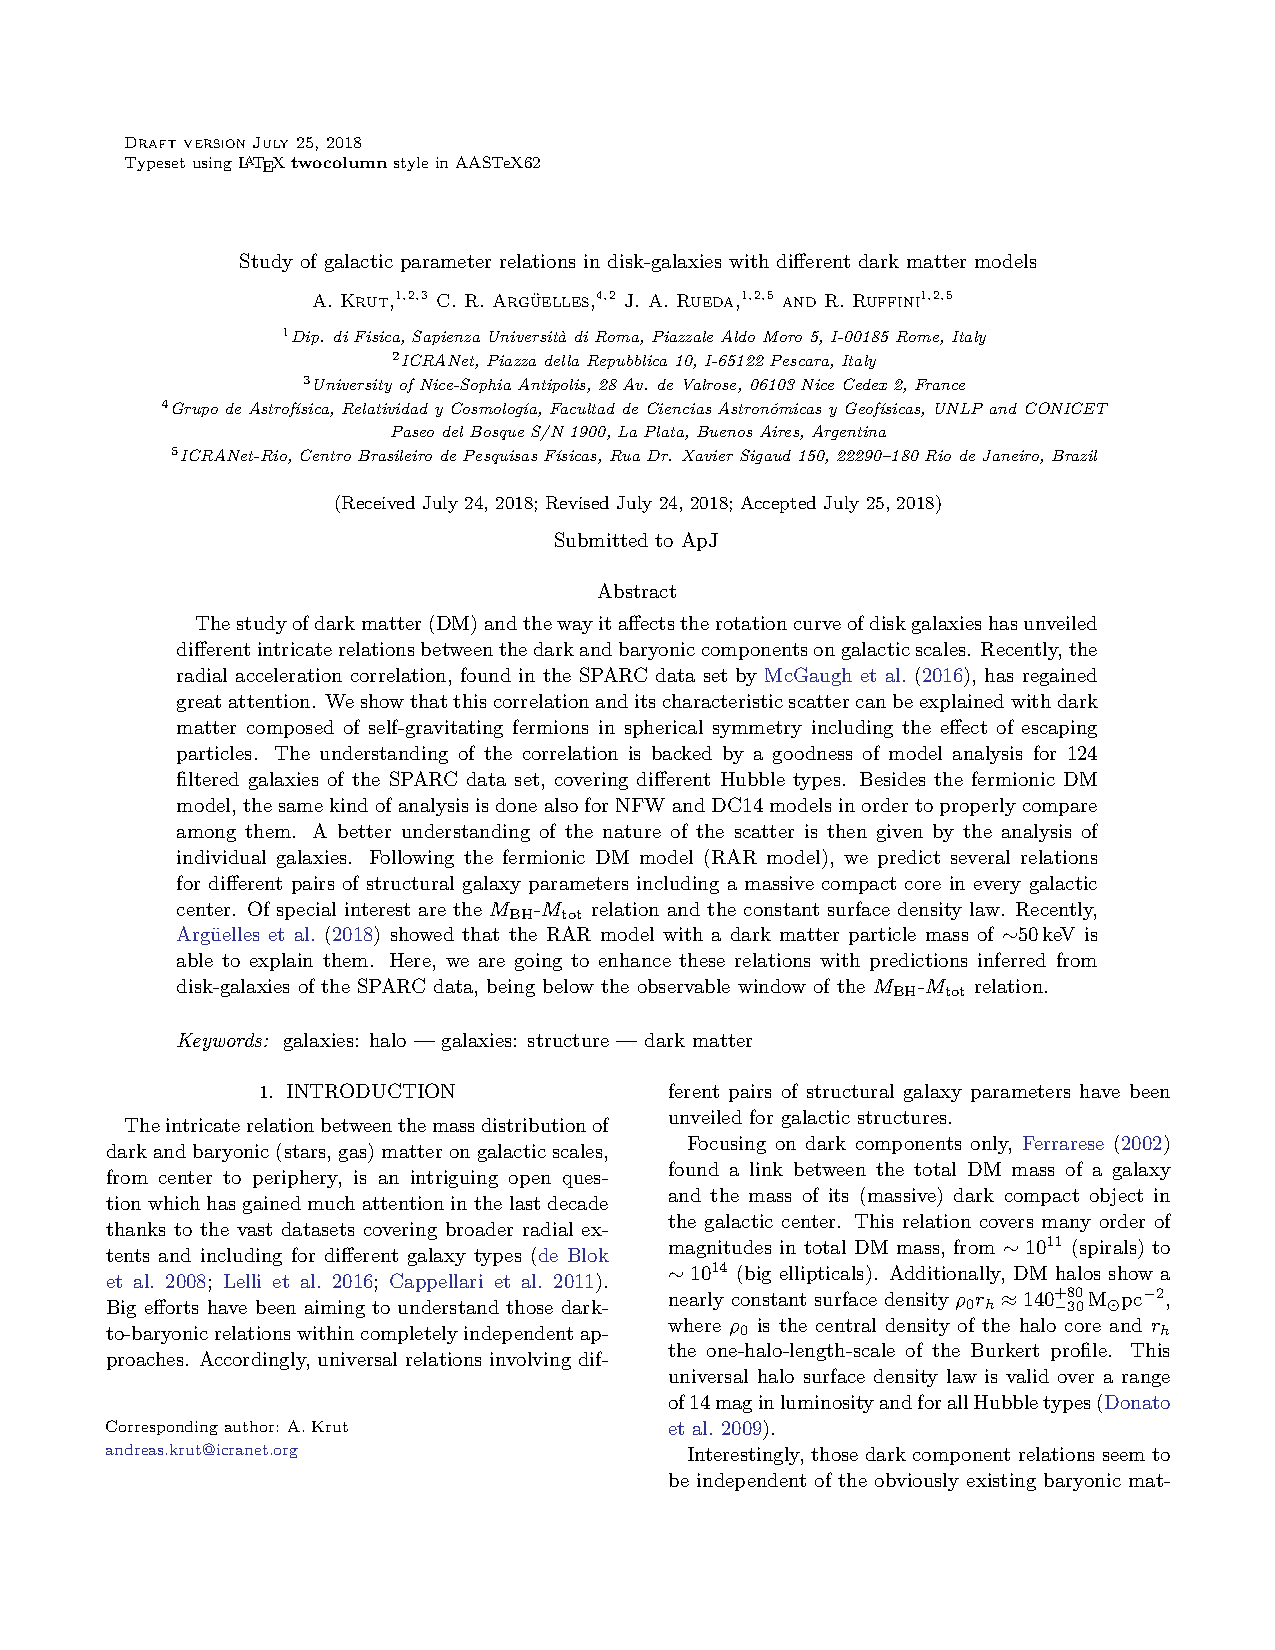
\includegraphics[width=\hsize]{\ROOTPATH/main.pdf}%
	\caption{Goodness of model analysis for the entire sample (120 galaxies). We count the population of fitted galaxies having a reduced $\chi^2$ smaller than a given one. The normalized population (step-like) follows nearly a log-normal distribution (solid) characterized by the mean value $\hat \chi^2_r$. The shaded regions span the $\SI{95}{\percent}$ confidence interval of the best-fitted $\hat \chi^2_r$.}%
	\label{fig:goodness:all}
\end{figure}